\documentclass{article}
\usepackage[T1]{fontenc}
\usepackage{lmodern}
\usepackage{graphicx}
\usepackage{amsmath,amssymb}
\usepackage[a4paper,margin=2cm]{geometry}
\usepackage[absolute,overlay]{textpos}
\setlength{\TPHorizModule}{1mm}
\setlength{\TPVertModule}{1mm}
\usepackage[indonesian]{babel}
\usepackage{hyperref}
\setlength{\emergencystretch}{2em}
% unit: Halaman 48

\begin{document}

% === Halaman 48 (llm) ===

\section*{Contoh 1:}

\begin{itemize}
    \item Tinjau 1 buah $pixel$ dari citra 24-bit ($3 \times 8$ bit):
    
    \begin{center}
        \color{red}10000010 \quad \color{red}01111011 \quad \color{red}01110101 \\
        (130) \quad (123) \quad (117)
    \end{center}

    \item Bit bit-bit $embedded\ message$: \color{blue}101
    
    \item $Embed$: \color{red}0011001\color{blue}1 \quad \color{red}1010001\color{blue}0 \quad \color{red}1110001\color{blue}1
\end{itemize}

\vspace{30mm}

Original: misalkan $pixel\ [130, 123, 117]$ berwarna ``ungu'' \\
Stego-image: $pixel\ [131, 122, 117]$ tetap ``ungu'' tapi berubah sangat sedikit. Mata manusia tidak dapat membedakan perubahan warna yang sangat kecil.

% deskripsi: Ilustrasi proses steganografi LSB pada pixel gambar, menunjukkan perubahan bit terakhir (LSB) dari warna original ke stego-image berdasarkan pesan 101.
% bbox normalisasi: [0.1430, 0.5660, 0.7680, 0.7880]
\begin{textblock*}{131.25mm}(30.03mm,168.10mm)
\noindent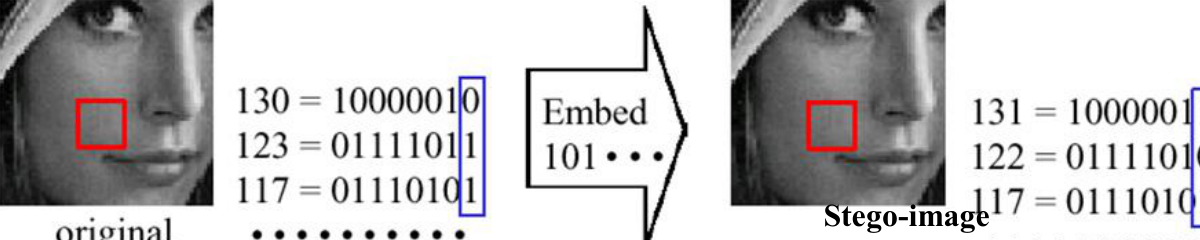
\includegraphics[width=131.25mm,height=65.93mm]{../../images/llm/page_048_img_01.png}%
\end{textblock*}

\end{document}
